\begin{frame}{Ejercicios}
\label{PolinomioLagrange}
\begin{Eje}[Ejercicio del examen del IIPA2023]
Sea $f(x)=\sqrt{x-x^2}$ y $P_2(x)$ el polinomio interpolante de Lagrange en $x_0=0$, $x_1$ y $x_2=1$. Calcule el valor de $x_1$ más grande en el intervalo $(0,1)$ para el cual $f(0.5)-P_2(0.5)=-0.25$ 
\end{Eje}
\small
Tip: evalúe en los puntos desde el inicio, así se sabe que términos se cancelaran.
$$f(x_0)=f(0)=0 \quad f(x_1)=\sqrt{x_1-x_1^2}\quad f(x_2)=f(x_1)=0$$
Parte I: Determine el polinomio de Lagrange
\begin{align*}
&P_2(x)\\
&=L_0(x)f(x_0)+L_1(x)f(x_1)+L_2(x)f(x_2)\\
&=\frac{(x-x_1)(x-x_2)}{(x_0-x_1)(x_0-x_2)}f(x_0)+\frac{(x-x_1)(x-x_2)}{(x_1-x_0)(x_1-x_2)}f(x_1)+\frac{(x-x_1)(x-x_2)}{(x_2-x_0)(x_2-x_1)}f(x_2)\\
&=\frac{(x-0)(x-1)}{(x_1-0)(x_1-1)}\sqrt{x_1-x_1^2}\\
&=\frac{x(x-1)}{x_1(x_1-1)}\sqrt{x_1-x_1^2}
\end{align*}
\end{frame}
%===========================
\begin{frame}{Ejercicios}
\small
Parte 2: Evalúe en 0.5
$$P_2(0.5)=\frac{0.5(0.5-1)}{x_1(x_1-0.5)}\sqrt{x_1-x_1^2}=-\frac{0.25\sqrt{x_1-x_1^2}}{x_1(x_1-1)}$$
Parte 3: Garantizar que $f(0.5)-P_2(0.5)=-0.25$ 
\begin{align*}
f(0.5)-P_2(0.5)&=-0.25\\
0.5+\frac{0.25\sqrt{x_1-x_1^2}}{x_1(x_1-1)}&=-0.25\\
\frac{0.5+0.25}{0.25}&=\frac{\sqrt{x_1-x_1^2}}{x_1(x_1-1)}\\
-3&=\frac{\sqrt{x_1(1-x_1)}}{-x_1(1-x_1)}=-\frac{1}{\sqrt{x_1(1-x_1)}}\\
9x_1(x_1-1)&=1\\
-9x_1^2+9x_1-1&=0 \quad \implies x=\frac{1}{2}\pm\frac{\sqrt{5}}{6}
\end{align*}
Por lo tanto, \textcolor{blue}{$x_1=\frac{1}{2}+\frac{\sqrt{5}}{6}\approx 0.8726779$\\} 
\hyperlink{RetornoPolinomioLagrange}{\textcolor{cyan}{Teoremas Preliminares.}}
\end{frame}
\begin{frame}{Ejercicios}
\begin{Eje}[Spline Cúbico]
Encuentre los splines cúbicos para la función $f(x)=\dfrac{1}{1+25x^2}$ en los puntos $\{x_0,\cdots,x_4\}=\{-1,-\dfrac{1}{2},0,\dfrac{1}{2},1\}$. Suponga condiciones naturales en -1 y fijas en 1.  
\end{Eje}	
\onslide<2->{\textcolor{red}{\indent Note que $h_j=\dfrac{1}{2}$ para todo $j$. Del númeral 5 en las fórmulas de recurrencia se obtiene que: 
\begin{align*}
\dfrac{3}{h_1}(a_{2}-a_1)-\dfrac{3}{h_0}(a_1-a_{0})=&h_{0}c_{0}+2(h_{0}+h_1)c_1+h_1c_{2}\\
\dfrac{3}{h_2}(a_{3}-a_2)-\dfrac{3}{h_1}(a_2-a_{1})=&h_{1}c_{1}+2(h_{1}+h_2)c_2+h_2c_{3}\\
\dfrac{3}{h_3}(a_{4}-a_3)-\dfrac{3}{h_2}(a_3-a_{2})=&h_{2}c_{2}+2(h_{2}+h_3)c_3+h_3c_{4}\\
\end{align*}}}
\end{frame}
%==========================================================================
\begin{frame}{Ejercicios}
\onslide<1->{\textcolor{blue}{\indent Sustituyendo los valores conocidos: 
\begin{align*}
6(f(0)-f(-1/2))-6(f(-1/2)-f(-1))=&c_{0}/2+2c_1+c_{2}/2\\
6(f(1/2)-f(0))-6(f(0)-f(-1/2))=&c_{1}/2+2c_2+c_{3}/2\\
6(f(1)-f(1/2))-6(f(1/2)-f(0))=&c_{2}/2+2c_3+c_{4}/2\\
\end{align*}}}
\onslide<2->{\textcolor{red}{\indent Simplificando: 
\begin{align*}
\dfrac{3450}{377}=&c_{0}+4c_1+c_{2}\\
-\dfrac{600}{29}=&c_{1}+4c_2+c_{3}\\
\dfrac{3450}{377}=&c_{2}+4c_4+c_{4}\\
\end{align*}}}
\onslide<3->{\textcolor{blue}{\indent En este punto se necesitan agregar las condiciones de frontera. Si se empieza por las naturales se tendría que $S''(-1)=S_0''(-1)=2c_0=0$, lo cuál implica que $c_0=0$.}}
\end{frame}
%==========================================================================
\begin{frame}{Ejercicios}
\onslide<1->{\textcolor{red}{\indent La condición en el extremo derecho exige que $f'(1)=-\dfrac{25}{338}=b_4$. Si se agrupan las últimas ecuaciones en las fórmulas de recurrencia, se obtendría:
\begin{align*}
a_{n}=&a_{n-1}+b_{n-1}h_{n-1}+c_{n-1}h_{n-1}^2+d_{n-1}h_{n-1}^3\\
b_n=&b_{n-1}+2c_{n-1}h_{n-1}+3d_{n-1}h_{n-1}^2\\
c_n=&c_{n-1}+3d_{n-1}h_{n-1}\\
\end{align*}
\indent Si se despeja $b_{n-1}$ y $d_{n-1}$ desde la segunda y tercera ecuación respectivamente y luego se sustituye y se simplifica en la primera ecuación, se obtiene que:
\begin{center}
$2h_{n-1}c_n+h_{n-1}c_{n-1}=\dfrac{3}{h_{n-1}}(a_{n-1}-a_{n})$, \ 
$2h_{3}c_4+h_{3}c_{3}=\dfrac{3}{h_{3}}(a_{3}-a_{4})$\\
\end{center}
Sustituyendo los valores conocidos se obtiene que:
$$c_4+c_3/2=6(f(1/2)-f(1)),\ 2c_4+c_3=\dfrac{450}{377}$$
}}
\end{frame}
%==========================================================================
\begin{frame}{Ejercicios}
\onslide<1->{\textcolor{blue}{\small\indent Juntando las condiciones de frontera obtenemos que: 
\begin{align*}
0=&c_0\\
\dfrac{450}{377}=&2c_4+c_3\\
\dfrac{3450}{377}=&c_{0}+4c_1+c_{2}\\
-\dfrac{600}{29}=&c_{1}+4c_2+c_{3}\\
\dfrac{3450}{377}=&c_{2}+4c_3+c_{4}
\end{align*}}}
\onslide<2->{\textcolor{red}{\small\indent Resolviendo el sistema anterior se obtiene que: 
\begin{align*}
[a_0,a_1,a_2,a_3,a_4]=&\bigg[\dfrac{1}{26},\dfrac{4}{29},1,\dfrac{4}{29},\dfrac{1}{26}\bigg]\\
[b_0,b_1,b_2,b_3]=&\bigg[-{{17850}\over{36569}},{{4425}\over{2813}},-{{1275}\over{36569}},-{{52425}\over{36569}}\bigg]\\
[c_0,c_1,c_2,c_3,c_4]=&\bigg[0,{{150750}\over{36569}},-{{268350}\over{36569}},{{166050}\over{36569}},-{{61200}\over{36569}}\bigg]\\
[d_0,d_1,d_2,d_3]=&\bigg[{{100500}\over{36569}},-{{279400}\over{36569}},{{289600}\over{36569}},-{{151500}\over{36569}}\bigg]\\
\end{align*}}}
\end{frame}
\begin{frame}{Ejercicios}
\begin{Eje}[Ejercicio de Richard Burden, Sección de trazadores cúbicos]
Un trazador cúbico sujeto $S$ de la función $f$ está definido por:
\begin{displaymath}
S(x)=
\left\{
\begin{matrix}
S_0(x)=1+Bx+2x^2-2x^3 & x\in[0,1]\\
S_1(x)=1+b(x-1)-4(x-1)^2+7(x-1)^3 & x\in[1,2]
\end{matrix}
\right.
\end{displaymath} 
Obtenga $f'(0)$ y $f'(2)$. 
\end{Eje}
\small
\onslide<2->{\textcolor{blue}{\indent Dado que estos representa trazadores cúbicos entonces se cumplen las siguientes condiciones:
$$S_0(1)=S_1(1)$$
$$S'_0(1)=S'_1(1)$$
}}
\onslide<3->{\textcolor{red}{\indent La primera ecuación deja como resultado:
$$1+B=S_0(1)=S_1(1)=1\Longrightarrow B=0.$$
La segunda ecuación dá como resultado:
$$-2=S'_0(1)=S'_1(1)=b\Longrightarrow b=-2.$$
Con esto se puede calcular $f'(0)=S'_0(0)=0$ y $f'(2)=S'_1(2)=11$.
}}
\end{frame}
\begin{frame}[fragile]{Ejercicios}
\begin{Eje}[Cota de error interpolación de Lagrange]
\indent Considere la siguiente función $f(x)=\sin(\ln(x)).$ Encuentre una cota para el error de aproximación del polinomio interpolante de Lagrange en el intervalo $[2,2.6]$ con tres puntos; $x_0=2$, $x_1=2.4$ y $x_2=2.6$. 
\end{Eje}
\action<+->{\ }
\begin{itemize}
\item \action<+->{\textcolor{red}{\indent Por el teorema relacionado con el polinomio de Lagrange, se sabe que:
$$|f(x)-P(x)|=\bigg|\dfrac{f^{(3)}(\xi(x))}{6}(x-2)(x-2.4)(x-2.6)\bigg|,$$
para $x\in[2,2.6]$ y $\xi(x)\in(2,2.6)$}}
\item \action<+->{\textcolor{red}{\indent Para encontrar las cotas sobre la tercera derivada se necesitan los siguientes cálculos:
\begin{align*}
f^{(3)}(z)=&\dfrac{3\sin(\ln(z))+\cos(\ln(z))}{z^3}\\
f^{(4)}(z)=&-\dfrac{10\sin(\ln(z))}{z^4}\\
\end{align*}}}
\end{itemize}
\end{frame}
\begin{frame}{Ejercicios}
\begin{itemize}
\item\action<+->{\textcolor{red}{\indent Si se analizan los lugares donde la derivada de la tercera derivada se hacen cero, entonces se obtiene la ecuación:
$$\sin(\ln(z))=0,$$
esta ecuación tiene como solución $z=e^{n\pi}$ donde $n\in\mathbb{Z}$. Para todo $n\in\mathbb{Z}$, $e^{n\pi}\notin [2,2.6]$ y por lo tanto los únicos valores extremos de la tercera derivada son 2 y 2.6.\\
\indent Evaluando la tercera derivada se obtiene que:
$$f^{(3)}(2)\approx 0.335765$$
$$f^{(3)}(2.6)\approx 0.1722$$
y por lo tanto se puede garantizar que:
$$|f^{(3)}(x)|\leq f^{(3)}(2)$$
para todo $x\in[2,2.6].$
}}
\item \action<+->{\textcolor{red}{\indent Defina ahora la otra parte para la cota de error:
$$g(x)\equiv(x-2)(x-2.4)(x-2.6)=\dfrac{25x^3-175x^2+406x-312}{25}$$
}}
\end{itemize}
\end{frame}
\begin{frame}{Ejercicios}
\begin{itemize}
\item \action<+->{\textcolor{red}{\indent Resolviendo para la ecuación de segundo grado:
$$g'(x)=0.$$
\indent Se obtiene que $x=\dfrac{35-\sqrt{7}}{15}$ (una de las dos raíces) es el lugar donde alcanza el valor más alto. Entonces:
$$|g(x)|\leq g\bigg(\dfrac{35-\sqrt{7}}{15}\bigg)$$
para toda $x\in[2,2.6]$.}}
\item \action<+->{\textcolor{red}{Finalmente:
\scriptsize
$$|f(x)-P(x)|=\bigg|\dfrac{f^{(3)}(\xi(x))}{6}(x-2)(x-2.4)(x-2.6)\bigg|
\leq g\bigg(\dfrac{35-\sqrt{7}}{15}\bigg)f^{(3)}(2)/6\approx 9.4574\times 10^{-4}$$
\normalsize
\indent La cota de error entonces es aproximadamente $9.5\times 10^{-4}$.}}
\end{itemize}
\end{frame}
\begin{frame}{Ejercicios}
\begin{Eje}[Ajuste lineal]
Considere el siguiente conjunto de datos:
\begin{center}
\begin{tabular}{ll}
\hline
$x_i$ & $y_i$\\\hline
1&6.612\\
2& 9.742\\
3& 10.455\\
4& 14.545\\
5& 17.293\\
6& 19.544\\
7& 21.279\\
8& 26.167\\
9& 28.341\\
10& 29.158\\\hline
\end{tabular}
\end{center}
Por medio del método de mínimos cuadrados encuentre la pendiente ($a_1$) y el intercepto ($a_0$) del ajuste lineal.
\end{Eje}
\end{frame}
\begin{frame}{Ejercicios}
\textcolor{red}{Después de plantear el problema con los datos anteriores se obtiene la siguiente gráfica:}
\begin{figure}
\centering
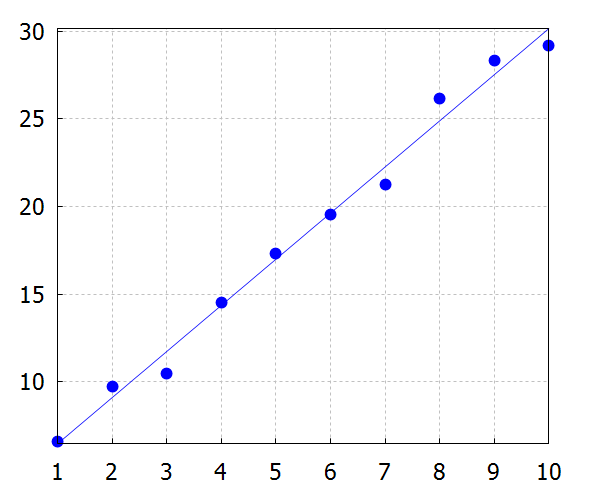
\includegraphics[scale=0.8]{Imagen23}
\caption{\textcolor{red}{En el ajuste se obtubieron los coeficientes $a_1=2.631$, $a_0=3.843$.}} 
\end{figure}
\end{frame}
\begin{frame}{Ejercicios}
\small
\begin{Eje}[Derivación de fórmula numérica]
Derive una fórmula de cinco puntos $O(h^4)$ para aproximar $f'(x)$ que utilice $f(x-h),f(x+h),f(x+2h),f(x+3h)$.  
\end{Eje}
\textcolor{red}{\indent El problema se puede plantear de la siguiente forma; encontrar constantes $A,B,C$ y $D$ tales que:
\begin{equation}\label{EjercicioAproximacionDerivada}
f'(x)= Af(x-h)+Bf(x+h)+Cf(x+2h)+Df(x+3h)+Ef(x).
\end{equation}
\indent Dado que se requiere una fórmula de orden 4, entonces se usará la fórmula de Taylor hasta el orden 5. Dejando de lado los residuos (estos tendrán como factor común a $h^5$), al hacer la suma y agrupar la parte derecha \eqref{EjercicioAproximacionDerivada} como un polinomio cuártico en términos de $h$, se obtienen los siguientes coeficientes:
\begin{itemize}
\item Coeficiente independiente: $(A+B+C+D+E)f(x)$.
\item Coeficiente de $h$: $(3D+2C+B-A)f'(x)$.
\item Coeficiente de $h^2$: $(9D+4C+B+A)/2f''(x)$.
\item Coeficiente de $h^3$: $(27D+8C+B-A)/6f^{(3)}(x)$.
\item Coeficiente de $h^4$: $(81D+16C+B+A)/24f^{(4)}(x)$.
\end{itemize}
\indent Para que se cumpla \eqref{EjercicioAproximacionDerivada} (salvo por los residuos producto del polinomio de Taylor) se impondrá que todos los coeficientes del polinomio cuártico sean cero con excepción de el coeficiente de $h$ y $h^0$ (ya que se desea que sea igual a $f'(x)$).}
\end{frame}
\begin{frame}{Ejercicios}
\textcolor{red}{
\indent 
El coeficiente de $h$, convenientemente se hace igual a  $\frac{1}{h}$ para que sea igual a $f'(x)$ en lado izquierdo de\eqref{EjercicioAproximacionDerivada}. El sistema que resulta de los planteamientos que se hicieron antes, queda expresado de la siguiente forma:
\begin{align*}
0=&E+D+C+B+A\\
\dfrac{1}{h}=&3D+2C+B-A\\
0=&9D+4C+B+A\\
0=&27D+8C+B-A\\
0=&81D+16C+B+A
\end{align*}
\indent Después de resolver el sistema obtenemos.
$$A=-\dfrac{1}{4h},B=\dfrac{3}{2h},C=-\dfrac{1}{2h},D=\dfrac{1}{12h},E=-\dfrac{5}{6h}.$$
\indent Sustituyendo se obtiene:
$$f'(x)\approx\dfrac{-3f(x-h)+18f(x+h)-6f(x+2h)+f(x+3h)-10f(x)}{12h}$$
}
\end{frame}
\begin{frame}{Ejercicios}
\label{EjercicioCuadraturaError}
\begin{Eje}[Regla del trapecio]
Por medio del teorema del valor medio y la cuadratura con polinomios de Lagrange, pruebe la regla del trapecio:
$$\int_a^b f(x)dx=\dfrac{h}{2}[f(b)+f(a)]-\dfrac{h^3}{12}f''(\xi)$$
Donde $h=b-a$, $\xi\in(a,b).$
\end{Eje}
\begin{displaymath}
\begin{array}{rl}
\displaystyle \int_a^b f(x)dx=&\textcolor{blue}{\displaystyle \int_{a}^{b} \dfrac{x-b}{a-b}f(a)+\dfrac{x-a}{b-a}f(b)dx}\\
&\displaystyle +\textcolor{red}{\dfrac{1}{2}\int_{a}^{b}f''(\xi(x))(x-a)(x-b)dx}\\\pause
=&\textcolor{blue}{\dfrac{b-a}{2}[f(a)+f(b)]}-\textcolor{red}{f''(\xi)\int_{a}^{b}(x-a)(x-b)dx}\\
=&\textcolor{blue}{\dfrac{b-a}{2}[f(a)+f(b)]}-\textcolor{red}{\dfrac{(b-a)^3}{6}f''(\xi)}.
\end{array}
\end{displaymath}
\hyperlink{CuadraturaTeoremaValorMedio}{\textcolor{cyan}{Regreso a Técnicas de Cuadraturas.}}
\end{frame}
\begin{frame}{Ejercicios}
\begin{Eje}[Cuadratura Gaussiana]
Encuentre la fórmula de cuadratura Gaussiana para $n=2$.
\end{Eje}
\textcolor{red}{Incialmente calculamos el polinomio de Legendre $P_2(x)$
\begin{displaymath}
\begin{array}{rl}
P_2(x)=&\dfrac{1}{2^2}\sum_{k=0}^{2}\binom{2}{k}^2(x+1)^{2-k}(x-1)^k\\\pause
=&\dfrac{1}{4}(\binom{2}{0}^2(x+1)^2(x-1)^0+\binom{2}{1}^2(x+1)(x-1)+\binom{2}{2}^2(x+1)^0(x-1)^2)\\\pause
=&\dfrac{1}{4}((x+1)^2+4(x+1)(x-1)+(x-1)^2)\\\pause
=&\dfrac{1}{4}(x^2+2x+1+4(x^2-1)+x^2-2x+1)\\\pause
=&\dfrac{1}{4}(6x^2-2)\\\pause
=&\dfrac{3}{2}x^2-\dfrac{1}{2}\\\pause
\end{array}
\end{displaymath}
De aquí se deduce que $x_1=\dfrac{1}{\sqrt{3}}$ y $x_2=-\dfrac{1}{\sqrt{3}}$.
}
\end{frame}
\begin{frame}{Ejercicios}
\textcolor{red}{
Por otro lado se deben calcular los $c_i$.
\begin{displaymath}
\begin{array}{rl}
c_1=&\int_{-1}^{1}\prod_{j=1,j\neq 1}^{2}\dfrac{x-x_j}{x_1-x_j}dx\\\pause
=&\int_{-1}^{1}\dfrac{x-x_2}{x_1-x_2}dx\\\pause
=&\int_{-1}^{1}\dfrac{x+\frac{1}{\sqrt{3}}}{\frac{1}{\sqrt{3}}+\frac{1}{\sqrt{3}}}dx\\\pause
=&\dfrac{\sqrt{3}}{2}[\dfrac{x^2}{2}+\dfrac{x}{\sqrt{3}}]_{-1}^{1}\\\pause
=&1.
\end{array}
\end{displaymath}
De forma similar se puede encontrar que $c_2=1$. De esta forma se obtiene la fórmula:
$$f\bigg(\dfrac{1}{\sqrt{3}}\bigg)+f\bigg(-\dfrac{1}{\sqrt{3}}\bigg)$$\pause
}
\textcolor{cyan}{Según el teorema, esta fórmula de cuadratura tiene precisión 3. En este sentido tiene el mismo grado de precisión que la regla de simpson con menos puntos.}
\end{frame}
\begin{frame}{Ejercicios}
\begin{Eje}[Cuadratura Gaussiana, continuación]
Utilice la fórmula de cuadratura anterior para encontrar:
$$\int_{0}^{\pi/4}\cos^2(x)dx$$
\end{Eje}
\textcolor{red}{Primero se necesita hacer el cambio de variable para que la integral quede definida en el intervalo de [-1,1]. Es bien conocido que el cambio de variable necesesario es:
$$x=\dfrac{1}{2}[(b-a)t+a+b]=\dfrac{1}{2}[\dfrac{\pi}{4}t+\dfrac{\pi}{4}]=\dfrac{\pi}{8}t+\dfrac{\pi}{8}$$
Con la fórmula anterior se obtiene lo siguiente:\pause
\begin{displaymath}
\begin{array}{rl}
\int_{0}^{\pi/4}\cos^2(x)dx=&\int_{-1}^{1}\cos^2(\dfrac{\pi}{8}t+\dfrac{\pi}{8})\dfrac{\pi}{8}dt\\\pause
\approx &\dfrac{\pi}{8}(\cos^2(\dfrac{\pi}{8\sqrt{3}}+\dfrac{\pi}{8})+\cos^2(-\dfrac{\pi}{8\sqrt{3}}+\dfrac{\pi}{8}))= 0.642317
\end{array}
\end{displaymath}
}
\end{frame}
\begin{frame}{Ejercicios}
\textcolor{red}{Por otro lado:
$$\int_{0}^{\pi/4}\cos^2(x)dx=[\dfrac{\sin(2x)}{4}+\dfrac{x}{2}]_{0}^{\pi/4}\approx 0.6426990816987241$$\pause
El error de aproximación se cálcula acontinuación:
$$E(cos^{2}(x))=3.8184610^{-4}$$
}
\begin{Eje}[Fórmula de cuadratura]
Determine las constantes $a,b,c,d$ y $e$ que producirán una fórmula de cuadratura:
$$\int_{-1}^{1}f(x)dx=af(-1)+bf(0)+cf(1)+df'(-1)+ef'(1)$$
cuya precisión es 4.
\end{Eje}
\end{frame}
\begin{frame}{Ejercicios}
\textcolor{red}{
\begin{displaymath}
\begin{array}{rl}
\int_{-1}^{1}1dx=2=&a+b+c\\\pause
\int_{-1}^{1}xdx=0=&-a+c+d+e\\\pause
\int_{-1}^{1}x^2dx=\dfrac{2}{3}=&a+c-2d+2e\\\pause
\int_{-1}^{1}x^3dx=0=&-a+c+3d+3e\\\pause
\int_{-1}^{1}x^4dx=\dfrac{2}{5}=&a+c-4d+4e\\\pause
\end{array}
\end{displaymath}
}
\textcolor{cyan}{Resolviendo este sistema se obtiene:\\
$$a=\dfrac{7}{15},b=\dfrac{16}{15},c=\dfrac{7}{15},d=\dfrac{1}{15},e=-\dfrac{1}{15}$$
}
\end{frame}
\begin{frame}{Ejercicios}
\small
\begin{Eje}[Regla compuesta del trapecio]
Determine los valores de $n$ y $h$ de manera que la integral:
$$\int_{0}^{2}\dfrac{1}{x+4}dx,$$ 
se pueda aproximar con una excatitud de $10^{-5}$ y calcule la aproximación. Aplique la regla compuesta del trapecio. 
\end{Eje}
\textcolor{cyan}{
\begin{displaymath}
\begin{array}{lrl}
&E(f)=\bigg|\dfrac{b-a}{12}h^2f''(\mu)\bigg|=&\bigg|\dfrac{2-0}{12}h^2\dfrac{2}{(\mu+4)^3}\bigg|\ \textcolor{red}{\bigg(f''(x)=\dfrac{2}{(x+4)^3}\bigg)}\\\pause
&=&\bigg|\dfrac{1}{3}h^2\dfrac{1}{(\mu+4)^3}\bigg|\ \textcolor{red}{\bigg(\dfrac{1}{(x+4)^3}\leq\dfrac{1}{4^3} \bigg)}\\\pause
&\leq &\bigg|\dfrac{1}{3}h^2\dfrac{1}{(4)^3}\bigg|\\\pause
&\leq &10^{-5}.\\\pause
\Rightarrow& h\leq & 10^{-5/2}2^3\sqrt{3}\\\pause
\Rightarrow& \dfrac{2}{n}=\dfrac{b-a}{n}=h\leq & 10^{-5/2}2^3\sqrt{3}\\\pause
\Rightarrow& 45.64354\leq & n\Rightarrow n=46.
\pause
\end{array}
\end{displaymath}
}
\end{frame}
\begin{frame}{Ejercicios}
\small
\textcolor{cyan}{
$$0.40546510810\approx \ln(6)-\ln(4)=\int_{0}^{2}\dfrac{dx}{x+4}\approx\textcolor{red}{(R.C.T.\ con\ n=46)} 0.405470577804$$
}
\end{frame}